\documentclass[a4paper,10pt,twocolumn]{article}

\usepackage[utf8x]{inputenc}
\usepackage[french]{babel}
\usepackage{graphicx,times}
\usepackage[T1]{fontenc}
\usepackage{amsmath}
\usepackage[font=footnotesize]{caption}
\usepackage{fancyhdr}
\usepackage[explicit]{titlesec}
\usepackage{hyperref}
%\usepackage[square,comma,numbers]{natbib}
\usepackage{tabularx}

\newcolumntype{L}[1]{>{\raggedright\arraybackslash}p{#1}}
\newcolumntype{C}[1]{>{\centering\arraybackslash}p{#1}}
\newcolumntype{R}[1]{>{\raggedleft\arraybackslash}p{#1}}

%\renewcommand{\bibsection}{}
%\def\bibfont{\footnotesize}
%\setlength{\bibsep}{0.2em}
%\setlength{\bibhang}{10em}

\hypersetup{colorlinks=true, urlcolor=blue, urlbordercolor={0 0 1}, citecolor=black, citebordercolor={1 1 1}}

\addto\captionsfrench{\def\figurename{Fig.}}
\addto\captionsfrench{\def\tablename{Tableau}}

\captionsetup[figure]{labelsep=period, justification=raggedright, singlelinecheck=false}
\captionsetup[table]{labelsep=period, justification=centering, singlelinecheck=false}

\parindent 10pt

\setlength{\voffset}{-1.3in}
\setlength{\topmargin}{1.25cm}
\setlength{\headheight}{1.125cm}
\setlength{\headsep}{0cm}

\setlength{\hoffset}{-1in}
\setlength{\oddsidemargin}{1.3cm}
\setlength{\evensidemargin}{1.3cm}

\setlength{\textheight}{25cm}%23.5
\setlength{\textwidth}{18.5cm}

\setlength{\headsep}{0.67cm}
\setlength{\columnwidth}{8.75cm}
\setlength{\columnsep}{0.63cm}

\setlength{\abovecaptionskip}{0em}
\setlength{\belowcaptionskip}{0em}

\titleformat{\section}
  {\normalfont}{\thesection.}{0.5em}{\MakeUppercase{#1}}
\titleformat{\subsection}
  {\normalfont\itshape}{\thesubsection.}{1.5em}{#1}
\titleformat{\subsubsection}
  {\normalfont\itshape}{\thesubsubsection.}{1.5em}{#1}
	
\titlespacing\section{0pt}{1em}{0.5em}
\titlespacing\subsection{0pt}{1em}{0.5em}
\titlespacing\subsubsection{0pt}{1em}{0.5em}

\fancyhf{}
\fancyhead[R]{\fontsize{8pt}{8pt}\selectfont \textbf{S}YMPOSIUM DE \textbf{G}ENIE \textbf{E}LECTRIQUE (SGE 2018), 3-5 JUILLET 2018, NANCY, FRANCE}
\renewcommand{\headrulewidth}{0pt}


\pagestyle{empty}


\title{
\fontsize{24pt}{24pt}\selectfont
Gestion d'énergie avec entrées incertaines : \\
quel algorithme choisir ?\\
Illustration pour une maison solaire
}

\newcommand\tsp[1]{\textsuperscript{#1}}

\author{
\fontsize{11pt}{11pt}\selectfont
Pierre HAESSIG\tsp{*}, Jesse James PRINCE AGBODJAN\tsp{*}, Romain BOURDAIS\tsp{*}, Hervé GUÉGUEN\tsp{*}\\
\fontsize{10pt}{10pt}\selectfont
\tsp{*}IETR, CentraleSupélec
}

\date{}


\begin{document}

\maketitle
\thispagestyle{fancy}


\fontsize{9pt}{9pt}\selectfont
\textbf{RÉSUME --
Le pilotage optimal des systèmes énergétiques nécessite l'emploi d'algorithmes
de gestion optimale.
Ces outils se rattachent à théories de disciplines variées (Automatique, Optimisation, Recheche Opérationnelle),
qui ont chacune leur spécificité tout en se recouvrant partiellement.
%
Il est donc difficile, pour la personne ``non initiée'', de saisir les principales caractéristiques
de chaque approche pour pouvoir les comparer et finalement trouver
quelles méthodes sont plus adaptées à un problème donné.
%
Nous proposons ici, sur un exemple simple de système photovoltaïque-stockage, de
comparer différentes méthodes en soulignant en particulier les investissements
en temps à prévoir :
temps pour la compréhension du cadre théorique,
temps pour la modélisation du problème dans ce cadre,
temps pour l'implémentation numérique et la validation des résultats.
Nous soulignons également quelques pièges typiques, comme l'optimisation
déterministe anticipative dans un contexte stochastique.
}\\

\textbf{\textit{Gestion d'énergie, Optimisation dynamique, Optimisation stochastique,
Commande prédictive, Programmation Dynamique}}

\fontsize{10pt}{10pt}\selectfont


\section{Introduction}

De très nombreux travaux de recherche portent sur le pilotage des systèmes énergétiques
pour optimiser leur fonctionnement.
Les méthodes employées sont variées (cf. partie \ref{s:opt_meth})
et certaines nécessite un bagage théorique qui pourrait rebuter effrayer
une personne issue d'une discipline ``physique'' (génie électrique, énergétique)
plutôt que ``numérique'' (automatique, recherche opérationnelle) où ces méthodes
sont souvent mises au point.
La mise en œuvre peut également est difficile et coûteuse en temps de calcul.
C'est malheureusement le cas en particulier des méthodes
a priori les plus performantes du point de vue de l'optimalité.


\section{Banc de test: maison solaire}

\subsection{Modèle de la maison solaire}

\begin{figure}[!ht]
        \begin{center}
                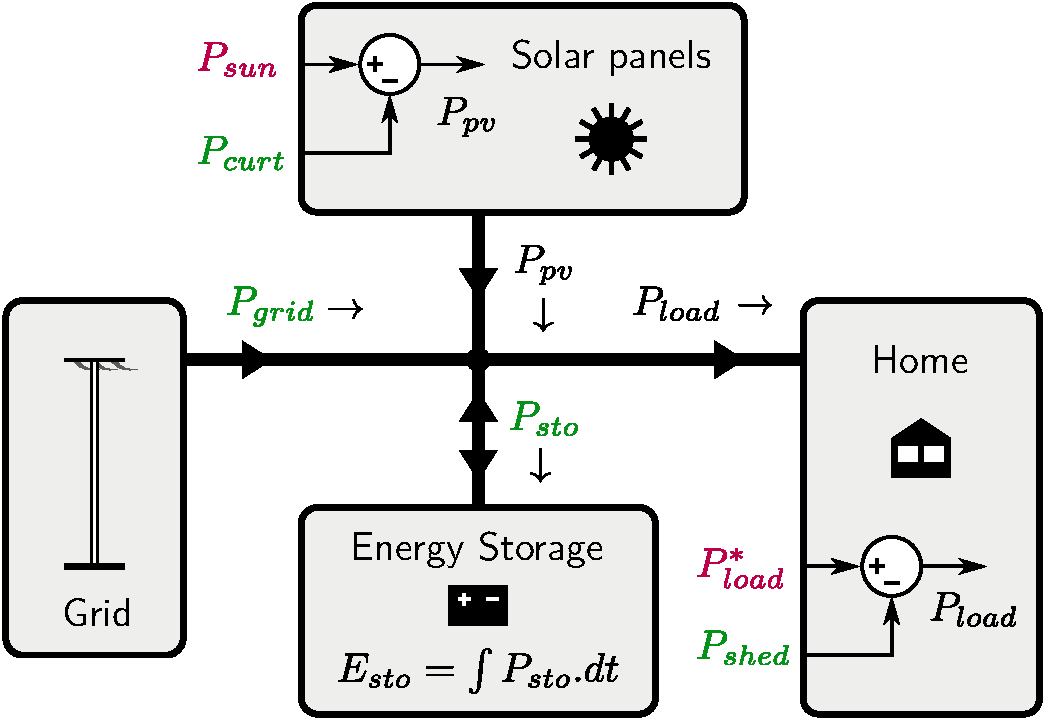
\includegraphics[width=0.9\columnwidth]{figures/solar_home.pdf}
        \end{center}

        \caption{Modèle en flux d'énergie de la maison solaire.
        Variables de décision en vert, données externes en rouge (potentiel solaire et consommation souhaitée), variables internes en noir.
        La consommation du foyer $P_{load}^*$, imposée, est couverte par 3 sources:
        le réseau électrique, des panneaux solaires (délestables)
        et un système de stockage.
        En dernier recours, la consommation de la maison peut être délestée.
        }
        \label{fig:solhome}
\end{figure}

Pour illustrer les différentes méthodes de gestion d'énergie à comparer,
nous avons choisi un système ``banc de test'' qui soit à la fois simple et concret.
Nous considérons ainsi la maison solaire qui est modélisée par
des flux d'énergie figure \ref{fig:solhome}.
Il s'agit d'un modèle simple de système photovoltaïque-stockage
pour l'autoconsommation d'un consommateur résidentiel connecté au réseau.

L'objectif de pilotage est la minimisation de la facture
de l'énergie consommmée du réseau ($\int P_{grid}$), le prix de l'énergie étant considéré fixe\footnote{un prix variable serait une extension naturelle}.
La puissance de réseau est limitée à la puissance souscrite $P_{grid}^{max}$
et l'injection est interdite\footnote{
équivalent, du point de vue de l'optimisation, à autoriser l'injection, mais sans la rémunérer}:
%
\begin{equation}
  0 \leq P_{grid} \leq P_{grid}^{max}
\end{equation}
%
Le système de gestion d'énergie doit donc tirer profit de l'énergie marginalement
gratuite des panneaux solaires $P_{pv}$, librement réglable entre 0 et $P_{sun}$
(par l'intermédiaire de l'écrêtage $P_{curt} \geq 0$).
$P_{sun}$ est le potentiel solaire maximal, obtenu lorsque les panneaux sont en régime
MPPT\footnote{Maximum power point tracking}) et qui est fonction de l'irradiance solaire du moment
ainsi que de la puissance nominale (puissance crête) des panneaux.

Le système de gestion doit également exploiter le degré de liberté offert par
le système de stockage qui permet de décaler, au moins partiellement,
la production solaire et la consommation. Le stockage, dont on néglige les pertes,
contient l'énergie:

\begin{equation}
  E_{sto}(t) = \int_0^t P_{sto}(t)dt
\end{equation}

Point essentiel, le stockage a une capacité limitée $E_{rated}$ :

\begin{equation}
  0 \leq E_{sto} \leq E_{rated}
\end{equation}

Tous les flux sont liés par la conservation de l'énergie:

\begin{equation}
  P_{grid} + P_{pv} = P_{load} + P_{sto}
\end{equation}

La consommation $P_{load}$ a vocation à suivre la consommation souhaitée $P_{load}^*$
(pas de charges ``intelligentes'' déplaçables). Nous définissons cependant un délestage de dernier
recours pour les situations critiques\footnote{faible puissance souscrite, lorsque
la batterie est vide et qu'il n'y a que peu de soleil}.

Notons pour finir que la performance d'un tel système dépend totalement de son dimensionnement
(capacité de stockage, puissance des panneaux et  puissance souscrite).
La question du dimensionnement, bien qu'intéressante, n'étant pas l'objet de cet article,
le dimensionnement est fixé empiriquement.

\subsection{Données de la maison solaire}

Ausgrid data :

\url{https://www.ausgrid.com.au/Common/About-us/Corporate-information/Data-to-share/Solar-home-electricity-data.aspx}

\url{https://github.com/pierre-haessig/ausgrid-solar-data}


\section{Approches d'optimisation}
\label{s:opt_meth}

TODO: cite thèse geeps voiture

\subsection{Programmation dynamique}
bon cadre théorique,

pb à l'implémentation

\cite{Haessig:2013:ESPy}

\subsection{Optimisation déterministe anticipative}
le piège

\cite{Rigo-Mariani:2014:SGE}

poster µgrid powertech 2015 ?

\subsection{MPC déterministe}
le classique

\subsection{MPC stochastique et robuste}

une amélioration du MPC déterministe.

\subsection{Commande prédictive non-linéaire}

Optimica JModelica.org \cite{Akesson:2010:CCE}

sareni sge 2014 \cite{Rigo-Mariani:2014:SGE} : optim linéaire puis reprojection.


\section{Conclusions}

Rappeler les principaux résultats marquants et originaux du travail. Le cas échéant, proposer des perspectives au travail présenté.

Perspectives : structure de décision dans un contexte multi-agent (pas abordé ici
car focus sur optimisation d'un système individuel) : centralisé, distribué,
mécanisme de prix, multi-agent...


\section{Remerciements}

Cette partie (facultative) doit être placée entre la conclusion et les références.


\bibliographystyle{IEEEtran}
\bibliography{00_References}


\end{document}

